\chapter{Tecnologie e strumenti}
\label{chap:tecno}

Durante lo sviluppo del progetto, sono state utilizzate varie tecnologie, strumenti, linguaggi e relativi framework che verranno dettagliatamente descritti di seguito.


\section{Microsoft Dial}
\begin{figure}[htpb!]
\center
  \includegraphics[width=0.2\textwidth]{Dial}
  \caption{Microsoft Dial}
\end{figure}
\section{Aulos}
\begin{figure}[htpb!]
\center
  
\includegraphics[width=0.2\textwidth]{LogoAulos}
  \caption{Aulos}
\end{figure}
AULOS è un framework ad uso interno per la standardizzazione dello sviluppo delle commesse.
Gli obiettivi principali di questo framework sono:
\begin{itemize}
\item rendere standard e subito disponibili quelle funzionalità che sono di frequente implementazione tra le commesse;
\item fornire uno standard UI e UX che sia ben riconoscibile, ma soprattutto coerente tra commesse diverse;
\item garantire l’interoperabilità tra tecnologie diverse.
\end{itemize}

AULOS fa uso di tecnologie web come Angular per il proprio frontend, mentre il backend – a cui esso si aggancia e che regola il funzionamento della commessa – può essere scritto in più linguaggi come C\# e LabView.
Da qui si nota come AULOS sia anche uno standard di comunicazione: l’utilizzo di API apre alla possibilità di sviluppare il backend nella tecnologia che meglio si sposa con il problema da risolvere.
\section{Angular}
\begin{figure}[htpb!]
\center
  
\includegraphics[width=0.2\textwidth]{LogoAngular}
  \caption{Angular}
\end{figure}
Angular 2+ (o semplicemente Angular) è un framework open source per lo sviluppo di applicazioni web con licenza MIT, evoluzione di AngularJS. Sviluppato principalmente da Google, la sua prima release è avvenuta il 14 settembre 2016.Angular è stato completamente riscritto rispetto a AngularJS e le due versioni non sono compatibili. Il linguaggio di programmazione usato per AngularJS è JavaScript mentre quello di Angular è TypeScript. Le applicazioni sviluppate in Angular vengono eseguite interamente dal web browser dopo essere state scaricate dal web server (elaborazione lato client). Questo comporta il risparmio di dover spedire indietro la pagina web al web-server ogni volta che c'è una richiesta di azione da parte dell'utente. Il codice generato da Angular gira su tutti i principali web browser moderni quali ad esempio Chrome, Microsoft Edge, Opera, Firefox, Safari ed altri. Angular è stato progettato per fornire uno strumento facile e veloce per sviluppare applicazioni che girano su qualunque piattaforma inclusi smartphone e tablet. Infatti le applicazioni web in Angular in combinazione con il toolkit open source Bootstrap diventano responsive, ossia il design del sito web si adatta in funzione alle dimensioni del dispositivo utilizzato. È in corso di sviluppo un altro toolkit di design responsivo, Flex Layout, più semplice da usare rispetto a Bootstrap e concepito appositamente per Angular. Altro toolkit che facilita la progettazione in Angular è Angular Material, una serie di componenti che permette di creare una pagina web molto velocemente: con l'utilizzo combinato di Flex Layout ed Angular Material si possono creare siti e applicazioni web responsive molto avanzate basate su Angular.
\section{TypeScript}
\begin{figure}[htpb!]
\center
  
\includegraphics[width=0.2\textwidth]{LogoTypescript}
  \caption{Typescript}
\end{figure}
TypeScript è un linguaggio di programmazione open source sviluppato da Microsoft. Si tratta di un Super-set di JavaScript che basa le sue caratteristiche su ECMAScript 6; capo del progetto è Anders Hejlsberg. Il linguaggio estende la sintassi di JavaScript in modo che qualunque programma scritto in JavaScript sia anche in grado di
16
funzionare con TypeScript senza nessuna modifica. È stato progettato per lo sviluppo di grandi applicazioni ed è destinato a essere compilato in JavaScript per poter essere interpretato da qualunque web browser o app.
\section{HTML}
\begin{figure}[htpb!]
\center
  
\includegraphics[width=0.2\textwidth]{LogoHTML}
  \caption{HTML}
\end{figure}
L'HTML è un linguaggio di pubblico dominio, la cui sintassi è stabilita dal World Wide Web Consortium (W3C). È derivato dall'SGML, un metalinguaggio finalizzato alla definizione di linguaggi utilizzabili per la stesura di documenti destinati alla trasmissione in formato elettronico. La versione attuale, la quinta, è stata rilasciata dal W3C nell'ottobre 2014. Il motivo principale che ha spinto il W3C e i suoi membri a sviluppare HTML5 è stata la necessità di fornire direttamente le funzionalità che in precedenza erano fruibili tramite estensioni proprietarie all'esterno dei browser, come Adobe Flash e simili. Un secondo obiettivo che gli sviluppatori si erano prefissati era quello di garantire una maggiore compatibilità tra i diversi browser, indipendentemente dalla piattaforma software utilizzata, e principalmente mirata all'espansione dei dispositivi mobili.
\section{KendoUI}
\begin{figure}[htpb!]
\center
  
\includegraphics[width=0.2\textwidth]{LogoKendo}
  \caption{KendoUI}
\end{figure}
Kendo UI e un framework integrale di interfaccia utente HTML5 per costruire applicazioni e siti web interattivi e ad alte prestazioni.
\section{Microsoft UWP}
\begin{figure}[htpb!]
\center
  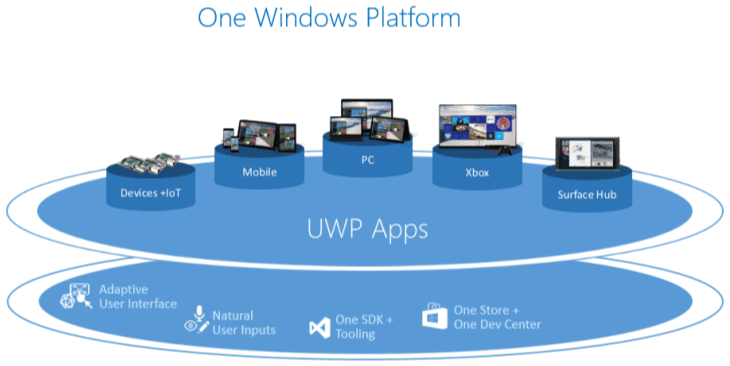
\includegraphics[width=0.2\textwidth]{LogoUWP}
  \caption{Microsoft UWP}
\end{figure}
UWP è uno dei numerosi modi per creare applicazioni client per Windows. Le app UWP usano le API WinRT per offrire potenti funzionalità avanzate di interfaccia utente e asincrone, ideali per i dispositivi connessi a Internet.
Per scaricare gli strumenti necessari per iniziare a creare le app UWP, vedere Effettuare la configurazione e quindi Scrivere la prima app ed è la soluzione ideale per creare app che vengono eseguite nei dispositivi Windows 10 e possono essere combinate con altre piattaforme. Le app UWP possono usare le API Win32 e le classi .NET (vedere Set di API per le app UWP, DLL per le app UWP e .NET per le app UWP).Il progetto di sviluppo Microsoft continua a evolversi e, insieme a iniziative come WinUI, MSIX e Project Reunion, UWP rappresenta uno strumento potente per la creazione di app client.
Un'app UWP è:
\begin{itemize}
\item Sicura: le app UWP dichiarano le risorse del dispositivo e i dati a cui accedono. L'utente deve autorizzare tale accesso.
\item In grado di usare un'API comune in tutti i dispositivi che eseguono Windows 10.
\item In grado di usare funzionalità specifiche del dispositivo e di adattare l'interfaccia utente alle dimensioni, alle risoluzioni e ai DPI dello schermo di dispositivi diversi.
\item Disponibile nel Microsoft Store in tutti i dispositivi (o solo a quelli specificati) che eseguono Windows 10. Il Microsoft Store offre diversi modi per realizzare profitti con un'app.
\item In grado di essere installata e disinstallata senza rischio o danni per il computer.
\item Coinvolgente: è possibile usare riquadri animati, notifiche push e attività utente che interagiscono con Sequenza temporale di Windows e la funzionalità di ripristino della ricerca dal punto in cui è stata interrotta di Cortana per coinvolgere gli utenti.
\item Programmabile in C\#, C++, Visual Basic e Javascript. Per l'interfaccia utente usare WinUI, XAML, HTML o DirectX
\end{itemize}
\section{C\#}
\begin{figure}[htpb!]
\center
  
\includegraphics[width=0.2\textwidth]{LogoC}
  \caption{C\#}
\end{figure}
Il C\# è un linguaggio di programmazione orientato agli oggetti sviluppato da Microsoft all'interno dell'iniziativa .NET, e successivamente approvato come standard dalla ECMA (ECMA-334) e ISO (norma ISO/IEC 23270).
La sintassi e struttura del C\# prendono spunto da vari linguaggi nati precedentemente, in particolare Delphi, C++, Java e Visual Basic.
\section{Libreria RadialController}
La libreria RadialController e le API correlate consentono di personalizzare sia il menù dei comandi integrato che l'esperienza di interazione supportata dall’ app.
Metodi utilizzati:
\begin{itemize}


\item RadialController.CreateForCurrentView()\\
Metodo statico che consente di ricevere un oggetto della classe RadialController creato appositamente per il contesto in cui gira l’applicazione (Dial utilizzato, versione del sistema operativo, tipo di hardware, ...)
\item .CreateFromIcon("Sample", icon)\\
Metodo che consente di creare un RadialControllerMenuItem ovvero un oggetto che inserito all’interno del menu verrà visualizzato e consentirà di svolgere un determinato comportamento quando selezionato.
\item .Menu.Items.
\begin{itemize}
\item Add(RadialControllerMenuItem item)
\item Inserisce il RadialControllerMenuItem all’interno del menu.
\item CreateFromKnownIcon(string displayText, RadialControllerMenuKnownIcon value)
\item Crea un oggetto di tipo RadialControllerMenuItem da un’icona già presente nella libreria.
\item CreateFromIcon(string displayText, RandomAccessStreamReference icon)
\item Crea un oggetto di tipo RadialControllerMenuItem da un’icona presente negli assets
\item CreateFromFontGlyph(string displayText, string glyph, string fontFamily)
\item Crea un oggetto di tipo RadialControllerMenuItem da un font installato nel sistema / inserito nell’app, e da un codice esadecimale ad esso associato
\end{itemize}
\end{itemize}
Eventi utilizzati:
\begin{itemize}
\item radialController.ButtonClicked\\
Evento che informa della pressione breve del dispositivo Dial.
\item radialController.ButtonPressed\\
Evento che informa della pressione prolungata del dispositivo Dial
\item radialController.RotationChanged\\
Evento che informa della rotazione del dispositivo Dial
\item .ScreenContactStarted\\
Evento che informa del posizionamento del Dial su schermo
\item .ScreenContactContinued\\
Evento che informa sull’utilizzo del Dial su schermo
\item .ScreenContactEnded\\
Evento che informa sulla fine del posizionamento su schermo
\end{itemize}
API correlate\\
RadialControllerConfiguration è una classe correlata alla classe RadialController e permette di configurare l’oggetto della medesima classe modificando le sue proprietà.\\
SetDefaultMenuItems consente di scegliere tra le voci di menù già predisposte dalla libreria quale inserire nel menù.

\section{Git}
\begin{figure}[htpb!]
\center
  
\includegraphics[width=0.2\textwidth]{LogoGit}
  \caption{Git}
\end{figure}
\section{GitLab}
\begin{figure}[htpb!]
\center
  
\includegraphics[width=0.2\textwidth]{LogoGitLab}
  \caption{GitLab}
\end{figure}
\section{Miro}
\begin{figure}[htpb!]
\center
  
\includegraphics[width=0.2\textwidth]{LogoMiro}
  \caption{Miro}
\end{figure}
\section{Teams}
\begin{figure}[htpb!]
\center
  
\includegraphics[width=0.2\textwidth]{LogoTeams}
  \caption{Teams}
\end{figure}
\section{Trello}
\begin{figure}[htpb!]
\center
  
\includegraphics[width=0.2\textwidth]{LogoTrello}
  \caption{Trello}
\end{figure}
\section{Visual Studio}
\begin{figure}[htpb!]
\center
  
\includegraphics[width=0.2\textwidth]{LogoVS}
  \caption{Visual Studio}
\end{figure}
\section{Remote Debugger}
\section{Visual Studio Code}
\begin{figure}[htpb!]
\center
  
\includegraphics[width=0.2\textwidth]{LogoVSCode}
  \caption{Visual Studio Code}
\end{figure}